\chapter{Persistent Homology and Contour Trees}
\label{chapter4}

We will now take a look at one of the tools that has made topological data analysis so viable in the recent years. This tool is called Persistent Homology (PH). It is primarily used for measuring topological features such as shapes. This is done by analysing the homology of subsets of the entire space. To accomodate this new concept we must first introduce some additional properties of the relations of homologies of topological spaces and their continous images. Following our theoretical foray we will examine the practical aspects of the computation of persistent homology and its relation to the computation and simplification of contour trees.

\section{Induced Maps on Homology}

Before introducing ourselves with persistent homology we will take a slight detour in order to introduce the last piece that we are missing to enable its construction. There is a general result in singular homology that shows the interaction of continuous maps and homomorphisms between homology groups.

\begin{defn} Let $X$ and $Y$ be two topological spaces. Let $f: X \to Y$ be a continuous function. Then $f$ induces a homomorphism $f_*: H_n(X) \to H_n(Y)$ for all $n \in \{0, 1, 2, ...\}$. \end{defn}

This means that if we have a continuous function between two spaces we can immediately associate the homology classes of $X$ to those of $Y$. All we have to do to obtain the induced map is to compose the simplices with the continuous function $f$. The details of this process are outlines in \cite{algebraic-topology}.


% @TODO WHY?!
This general result is not appropriate for simplicial complexes. WHY?! We need a more tracktable definition to aid us in our computation. We will thus present the following combinatorially flavoured definition given by \cite{combinatorial-algebraic-topology}. 


\begin{defn} Let $X$ and $Y$ be two finite abstract simplicial complexes. A function $f: X \to Y$ is a simplical map when if $\sigma$ is a simplex of $X$ then $f(\sigma)$ is a simplex of $Y$. \end{defn}

The two most important observations we can make based on this defitions are the following:

\begin{itemize}
    \item The composition of two simplicial maps is simplicial.
    \item When $Y$ is a subcompex of $X$ the inclusion map is a simplicial map.
\end{itemize}


% @TODO Define a homology class
The reason why we introduced simplicial maps is so that we can pose the following question. If there is a simplical map between two simplicial complexes, can we use it to relate their homology classes? The answer is yes, we can thanks to \cite{combinatorial-algebraic-topology}!


% @TODO Are simplicial maps continuous?

\begin{defn} Let $X$ and $Y$ be two simplical complexes and $f: X \to Y$ be a simplicial map. Then $f$ induces a homomorphism $f_*: H_n(X) \to H_n(Y)$ for all $n \in \{0, 1, 2, ...\}$. \end{defn}

The homomorphism is induces by taking the simplicies of a chain through the simplicial map and the considering the homology class the chain ends up in (if any). Detail on this can be found in \cite{combinatorial-algebraic-topology}.

We will further expand this definition to also cover relative chain maps and relative homologies.

\begin{defn} Let $X$ and $Y$ be two simplical complexes and let $A \subseteq X$ and $B \subseteq Y$ be two subcomplexes. Let $f: X \to Y$ be a simplicial map such that $f(A) \subseteq B$. Then $f$ induces a homomorphism $f_*: H_n(X, A) \to H_n(Y, B)$ for all $n \in \{0, 1, 2, ...\}$. \end{defn}

We will use the shorthand $f: (X, A) \to (Y, B)$ for functions that satisfy the criteria of this definition. The function $f$ is called this a simplicial map between simplicial pairs (analogous to continuous map between topological pairs in \cite{algebraic-topology}). 


% @TODO Define absolute homology
The homomorphism is induced by running the relative homology classes through the simplicial map and recording which class their image lands in. The primary type of map we will use in this chapter is a specific kind of simplicial map - the inclusion map. The reason for this will become clear in the following section. In the case of absolute homology when $X$ is a simplicial complex and $A$ is a subcomplex of $X$ there is a natural inclusion map $i: A \to X$ which is injective but not necessarily surjective. It takes the simplicies of $A$ to exactly the same simplicies of $X$ and leaves the simplicies outside of $A$ untouched. 

We shall define the inclusion of relative homology analogously. Let $B$ be another subcomplex of $X$ such that $A$ is also a subcomplex of $B$, or $A \subseteq B \subseteq X$. Then let $i : X \to X$ be the identity map. As $A \subseteq B$ then the restriction $i_A: A \to B$ is a well defined function and therefore $i(A) \subseteq B$. Therefore there is a map $i$ between the pairs $(X, A)$ and $(X, B)$ such that $i(A) \subseteq B$ by the previous definition this map induces a homomorphism $i_* : H_n(X, A) \to H_n(X, B)$.


% @TODO Should I talk about chain maps?
% @TODO Add proof for all of this?

\section{Persistent Homology}

% @TODO Define filtrations.
% @TODO Introduce filtrations and VR complexes.

Persistent Homology emerged in the early 2000s in the this work of \cite{persistence-original}. The original motivation for introducing it was to better model point cloud data through filtrations of Vietoris Ribs complexes. Persistent Homology has since grown into a general methodology that can be applied any filtration of a topological space. To best illustrate what persistent homology is let us consider a filtration of a simplical complex $X$. 

$$ X_0 \subseteq X_1 \subseteq ... \subseteq X_{n-1} \subseteq X_n = X$$

A concrete example of this is Figure \ref{fig:filt-sc}.


\begin{figure}%
    \centering
    
\includegraphics[scale=0.085]{./images/chapter4/example-filtration.eps}%
    \caption{Filtration of a Simplical Complex}%
    \label{fig:filt-sc}%
\end{figure}

We have obtained a one parameter sequence of nester subcomplexes. Another way to think of this is that we start with simplicial complex and iteratively add new simplicies to it. It is customary to call the index of this filtration time to make it more indicative of a process that evolves in time. We can already compute the homology groups of the individual $X_i$. The key insight in persistent homology was to as the question whether we can track the evolution of individual homology classes in the homology groups as we go from one complex to the next. This is made possible by the subset relation between all of the $X_i$. As discussed in the previous section the inclusion map is the natural map between a set and it's superset. More formally we have inclusion maps $i_{i, j}: X_i \to X_j$ for $i \le j$ because $X_i \subseteq X_{i+1} \subseteq ... \subseteq X_j$. 
By only considering the inclusion maps between consecutive $X_i$ and $X_{i+1}$ we can build the following chain of simplicial complexes


$$ X_0 \overset{i}{\longrightarrow} X_1 \overset{i}{\longrightarrow} ... \overset{i}{\longrightarrow} X_{n-1} \overset{i}{\longrightarrow} X_n$$


% @TODO Introduce Chain Maps
where we have renamed all inclusion maps to $i$ and infer them from context. We have already shown that the inclusion maps are simplical and that simplical maps induce homomorphisms on homology groups through chain maps inducing. This lets us transform the sequence directly to the homology groups like so:

$$ H_n(X_0) \overset{i_*}{\longrightarrow} H_n(X_1) \overset{i_*}{\longrightarrow} ... \overset{i_*}{\longrightarrow} H_n(X_{n-1}) \overset{i_*}{\longrightarrow} H_n(X_n).$$

Here it is important to note that the induced maps $i_*$ do not have to be the inclusion maps on the homology groups. They can easily fail to be injective when for example two homology classes in some $H_n(X_i)$ map to the same homology class $H_n(X_{i+1})$ due to the introduction of a new boundary. This contradicts the fact that inclusion maps are injective. The induces homomorphisms encode the local topological changes in the homology of consecutive complexes in the filtration. We will introduce the following terminology to help us interpret this information:


% @TODO You may not be right about death here
\begin{itemize}
    \item A homology class is \textbf{born} if it is not the image of a class in the previous complex in the filtration under $i_*$.
    \item A homology class \textbf{dies} if its image under $i_*$ is the zero element or when it is merged with another class (they have the same iamge).
    \item A homology class \textbf{persists} if its image under $i_*$ is not zero.
\end{itemize}

In order to produce a detailed computation of the persistent homology of a filtration we would have to compute all homology groups of all complexes and then compute all inclusion maps. Doing so by hand is cumbersome and more importantly far too lengthy. We will avoid doing it in favour of presented diagrams of the evolution of the homology classes and appeal to the reader's geometric and topological intuition to argue their correctness.

*Let us look at the following example. Show a pretty picture and explain it*

Given the persistence homology of a filtration we can pose the question of how we can rank the classes based on their "significance". We are most interested in the classes that persist for a large number of steps in the filtration. Such classes are exactly the ones we consider significant and are said to have high persistence. Ephemeral classes on the other hand are consider to have very low significance and can be neglected. In practise such classes often correspond to statistical noise or sampling error.


% @TODO Should you add X_i here istead of just t_i?

To quantify this precisely we will produce the so called persistence pairs. A persistence pair $(t_1, t_2)$ is a pairing of two timestamps - the birth and death time of a homology class. Every class is associated with a pair such as this where $t_1$ is the birth time, $t_2$ is the death time and the class has persisted in all $t_1 \le t_i \le t_2$. In the cases of classes that never die such as *this one in that example* we will assume that their death time is $\infty$. We will call such classes essential and others inessential as in \cite{comp-topo}.

% @TODO Why is this true?
There is a theorem that states that the persistence digram of a filtration encodes all of the information about the persistent homology groups.

*Examples*

Finally we will describe an algorithm for computing the persistence pairs. It requires us order all of the simplices in the complex $\sigma_1, \sigma_2, ..., \sigma_n$ according to these rules \cite{ph-a-survey}.

\begin{itemize}
    \item $\sigma_i$ precedes $\sigma_j$ when $\sigma_j$ was introduced later in the filtration than $\sigma_i$
    \item $\sigma_i$ precedes $\sigma_j$ when $\sigma_i$ is a face of $\sigma_j$
\end{itemize}

Not instead of having to compute the homology groups of all complexes in the filtration individually and then computing the induces maps we can perform the whole computation in a single matrix reduction. Let $D$ be an $n\times n$ matrix and such that.

   $$
   D[i, j] = \left\{
       \begin{array}{@{}l@{\thinspace}l}
           \text{1}  &: \text{if } \sigma_i \text{ is a codimension 1 face of } \sigma_j \\
           \text{0}  &: \text{otherwise} \\
       \end{array}
   \right.
   $$

In other matrix $D$ is a matrix that holds the boundaries of all simplicies in a single matrix. It is called the combined boundary matrix. Now we can perform the following reduction just by column operations.


\begin{algorithm}
\caption{Reduce Combined Boundary Matrix}

\begin{algorithmic}[1]


\ForAll {j $\in$ \{1, 2, ..., n\}} 
    \While {$\exists j': j' < j \text{ and } low(j') == low(j) $}
        \State Add column $j'$ to column $j$.
    \EndWhile
\EndFor

\end{algorithmic}
\end{algorithm}

The proof of this algorithm is outlined in \cite{persistence-original}.

% @TODO What kind does the manifold have to be?
Now let us apply this general theory to a Morse theoretic context. Let $M$ be a triangulation of a smoothly embeded 2-manifold in $\mathbb{R}^3$ and let $f : M \to \mathbb{R}$ be a Morse function. From Morse theory we know that the changes in topology can only happen at finitely many critical points of $M$. Let $c_1 < c_2 < ... < c_n$ be those critical points. Let us now use the sublevel sets $M_{c_i}$  to make a filtration of $M$.We obtain the following filtration which we will call ascending

$$ M_{c_1} \subseteq M_{c_2} \subseteq ... \subseteq M_{c_{n-1}} \subseteq M_{c_n} = M.$$

From this filtration we can produce the following persistent homology chain

$$ H_n(M_{c_1}) \overset{i_*}{\longrightarrow} H_n(M_{c_2}) \overset{i_*}{\longrightarrow} ... \overset{i_*}{\longrightarrow} H_n(M_{c_{n-1}}) \overset{i_*}{\longrightarrow} H_n(M_{c_n}) = H_n(M).$$

If we had taken the superlevel sets of $M$ we would have obtained a different filtration. We will call that the descending filtration of $M$.

$$ H_n(M^{c_1}) \overset{i_*}{\longrightarrow} H_n(M^{c_2}) \overset{i_*}{\longrightarrow} ... \overset{i_*}{\longrightarrow} H_n(M^{c_{n-1}}) \overset{i_*}{\longrightarrow} H_n(M^{c_n}) = H_n(M).$$




Finally we will define what we call the persistence of a homology class.

\begin{defn} The persistence of a single homology class in persistent homology that is born at time $t_1$ and dies at time $t_2$ is $t_1 - t_2$.  \end{defn}

% @TODO Do this
    There are two primary ways to visualize the persistence pairing produces by persistent homology. The first in through persistence diagrams \cite{comp-topo}. In the persistence diagrams the pairs are visualised as points in the Carthesian coordinate system above the main diagonal $y = x$. Example []. The second way is through barcode diagrams. You can see the barcode digram on fig[]. For every simplical complex in the filtration we have a number of starting lines equal to the number of generators for the homology classes. These lines feed into each other according to where the induced by inclusion homomorphism take them in the next simplical complex. 

\begin{figure}[h]%
    \centering
    \includegraphics[scale=0.085]{./images/chapter4/bar-diagram.eps}%
    \caption{Barcode Diagram of a Filtration}%
    \label{fig:bar-diag}%
\end{figure}

\begin{figure}[h]%
    \centering
    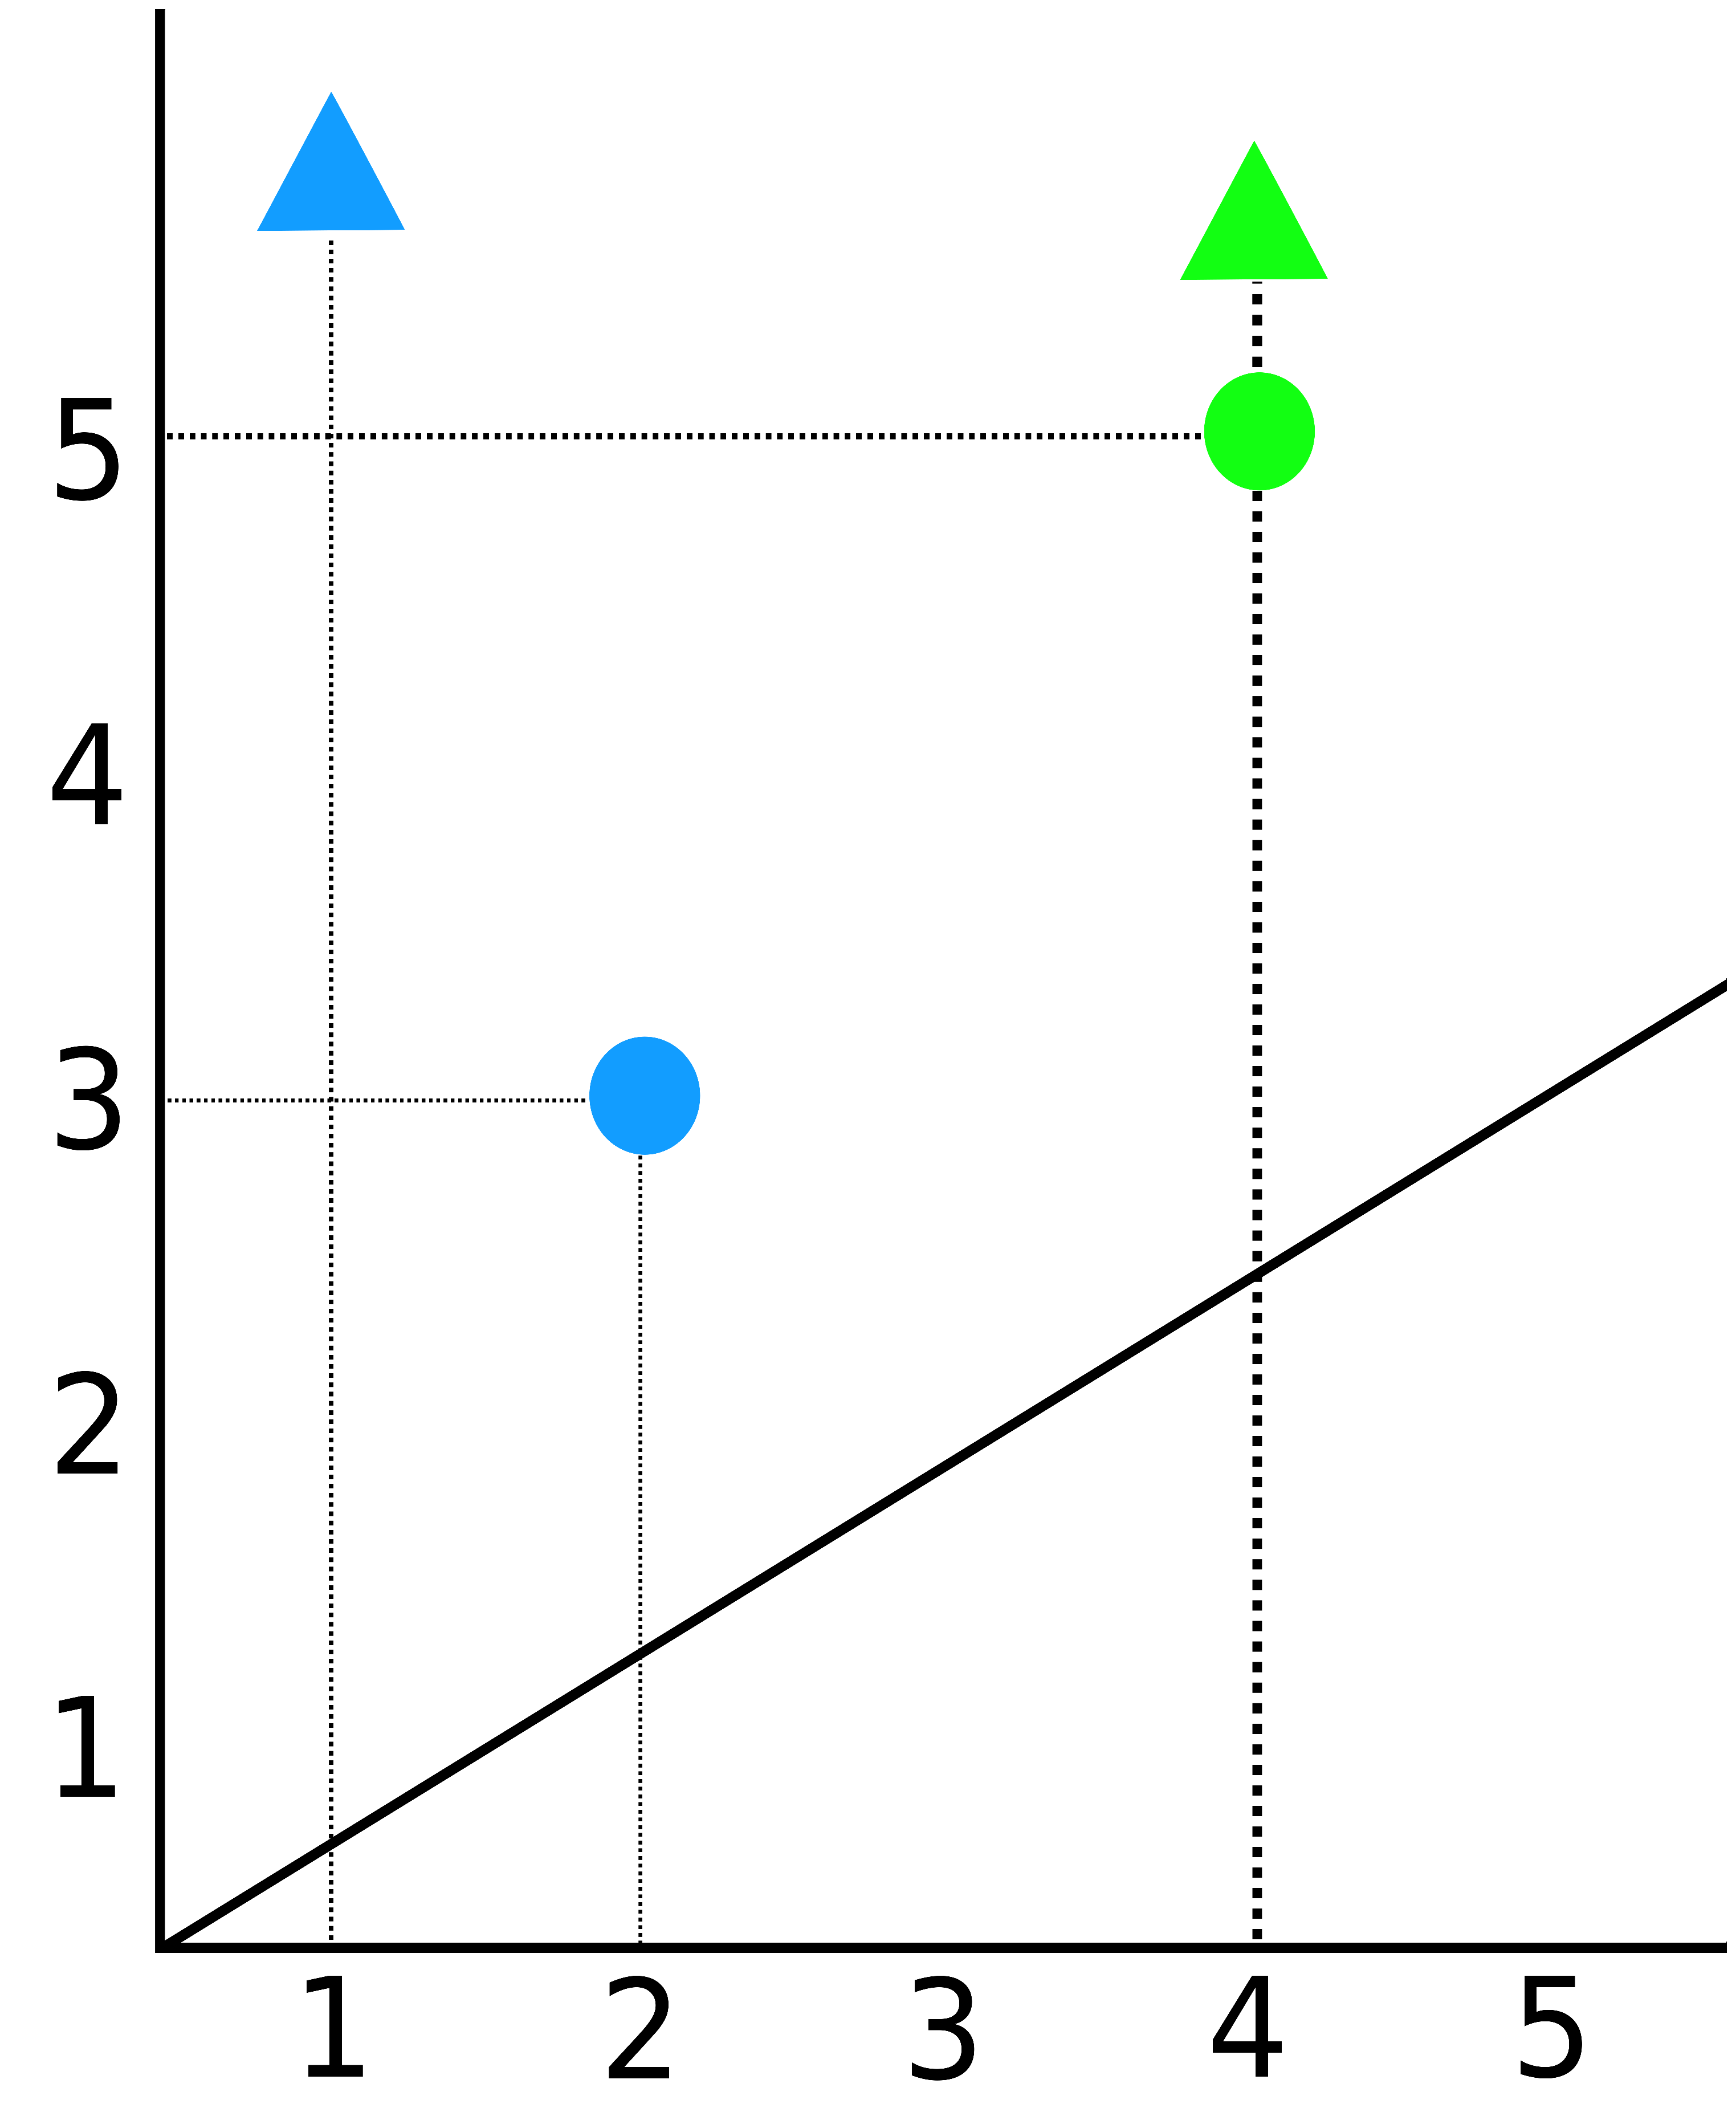
\includegraphics[scale=0.085]{./images/chapter4/diagram.eps}%
    \caption{Persistence Diagram of a Filtration}%
    \label{fig:per-diag}%
\end{figure}


% @TODO Add reference
Furthermore when two classes merge we must choose which one survives and which one dies. By established convention [] we will use the Elder Rule. By the Elder Rule the class that was born first continues to persistent and the younger one is destroyed.


%Here are two examples of filtrations and explanations of bar diagrams.


%Let us now restrict $M$ to be compact and contractable. This will ensure that the Reeb Graph of $M$ is a Contour Tree. We would like to tackle the claim made in \cite{ct-branch-decomp} that the persistent homology pairs are equivalent to branch decomposition pairs. We can immediately see that this claim is either false of ill-defined. The major reason for this is that essential homology classes do not get paired. But in the branch decomposition schemes all critical points are paired.

%There is however yet more reason to pursue this. Slightly after the paper of branch decomposition was published, there emerged a way to extend the persistent homology scheme so that all critical points get paired. Using this will allows us to directly compare it to the branch decomposition of a contour tree. 

%We will now show that computing the persistent homology of the descending and ascending filtration of $M$ is equivalent to constructing the join and split tree of $M$ respectively.

%* Show that this is the case *

%* SHOW EXAMPLES *

% Define extended persistence.

\section{Extended Persistence}

*CAN THE SAME CRITICAL POINT BE TWO TWINGS?*

We have seen from the definition and computations of persistent homology that not all critical points are paired. Those that give birth the essential persistent homology classes will not be paired because they are never destroyed pass the final simplex in the filtration. This leads to incompleteness in the persistence pairings which we would to remedy. Our goal in extending persistence it to find a natural and intuitive way to pair the essential homology classes. In terms of filtrations of triangulations of manifolds based on the sub/superlevel sets of a Morse functions this means that all critical points will be paired in some homology.

*SHOW EXAMPLE*

* REDO FIRST SENTENCE *
The way we have paired the remaining critical points in the above example is hopefully both symmetric and consistent with our intuition (developed in the example above). But how do we justify doing so theoretically? Enter extended persistence. The main idea behind extended persistence is to follow the ascending pass of persistent homology with a descending pass where once we reach a class that is homologous to a essential class in the ascending filtration we consider it to be destroyed and thus paired. To justify this algebraically we would like to make this process a consequence of a new augmented chain that starts with the zero homology group and ends with the zero group. This way we have an assurance that every class that is born will eventually die.

Our initial instinct here might be to just directly apply persistent homology twice. Once on the ascending and the on the descending filtration. The problem that arises is in relating the classes of the two different filtrations. We are able to merge both filtrations into a single long chain, but the induced maps of the two filtrations flow in different directions. Here is an example of what would happen if we attempt this

$$ 0 = H_n(M_{c_1}) \rightarrow ... \rightarrow H_n(M_{c_n}) = H_n(M) = H_n(M^{c_1}) \leftarrow ... \leftarrow H_n(M^{c_{n}}) = 0.$$

The direction of the arrows is accordance with the how the homomorphisms are induced. To verify this consider that $M_{c_i} \subseteq M_{c_j}$ and $M^{c_j} \supseteq M^{c_j}$ for $i \le j$. This can be remedied if we find a way to reverse the directions of the arrows in the descending filtration. The issue in finding new maps to induce homomorphisms in the opposite direction is that we will sacrifice the our intuition which captures the evolution of homology classes. This is because other induced homomorphisms will not be natural and as such will be harder to interpret. If we wish to keep using natural inclusion maps we must instead resort to changing the homology groups we use. Let us opt for a descending filtration of relative homology groups like so:

$$ H_n(M) = H_n(M, M^{c_n}) \rightarrow H_n(M, M^{c_{n - 1}}) \rightarrow ... \rightarrow H_n(M, M^{c_{1}}) = 0 $$


% @TODO By which def (end of paragraph)
In this relative filtration the homomorphisms are induced by inclusions on the relative homology groups. To see this let $(M, M^{c_i})$ and $(M, M^{c_{i+1}})$ two consecutive pairs. The inclusion map from $M$ to $M$ takes the superlevel set $M^{c_i}$ in the superlevel set $M^{c_{i+1}}$ because $M^{c_i} \subseteq M^{c_{i+1}}$. By definition [] this is a simplicial map from $(M, M^{c_i})$ and $(M, M^{c_{i+1}})$ and thus induces a homomorphism between $H_n(M, M^{c_i})$ and $H_n(M, M^{c_{i+1}})$.

The final step to complete our desired sequence is to "glue" these two filtrations together at the point $ H_n(M_{c_n}) = H_n(M) = H_n(M, M^{c_n})$. The second equality holds because $M^{c_n} = \emptyset$ and quotienting by the empty set leaves the underlying relative chain complexes unchanged. Putting this all together yields the following chain of homology groups.

$$ 0 = H_n(M_{c_1}) \rightarrow ... \rightarrow H_n(M_{c_n}) = H_n(M) = H_n(M, M^{c_n}) \rightarrow ... \rightarrow H_n(M, M^{c_{1}}) = 0.$$

% @TODO Is that really what a close subcomplex is?

This augmented filtration justifies the pairing of essential classes according to the intuitive understanding we obtained from example []. The only issue is that the relative homology groups are difficult to interpret on their own. To aid our comprehension of what exactly occurs in the relative filtration we shall employ the Excision Theorem where $H_n(M, M^{c_i}) = H_0(M / M^{c_i}, pt) = \overset{\sim}{H}_0(M / M^{c_i})$ where $M^{c_i}$ is a closed subcomplex of $M$ as required for all $i \in \{1, 2, 3, ..., n\}$. 

* Take a look at example how the complex is built and the how it unwinds itself *

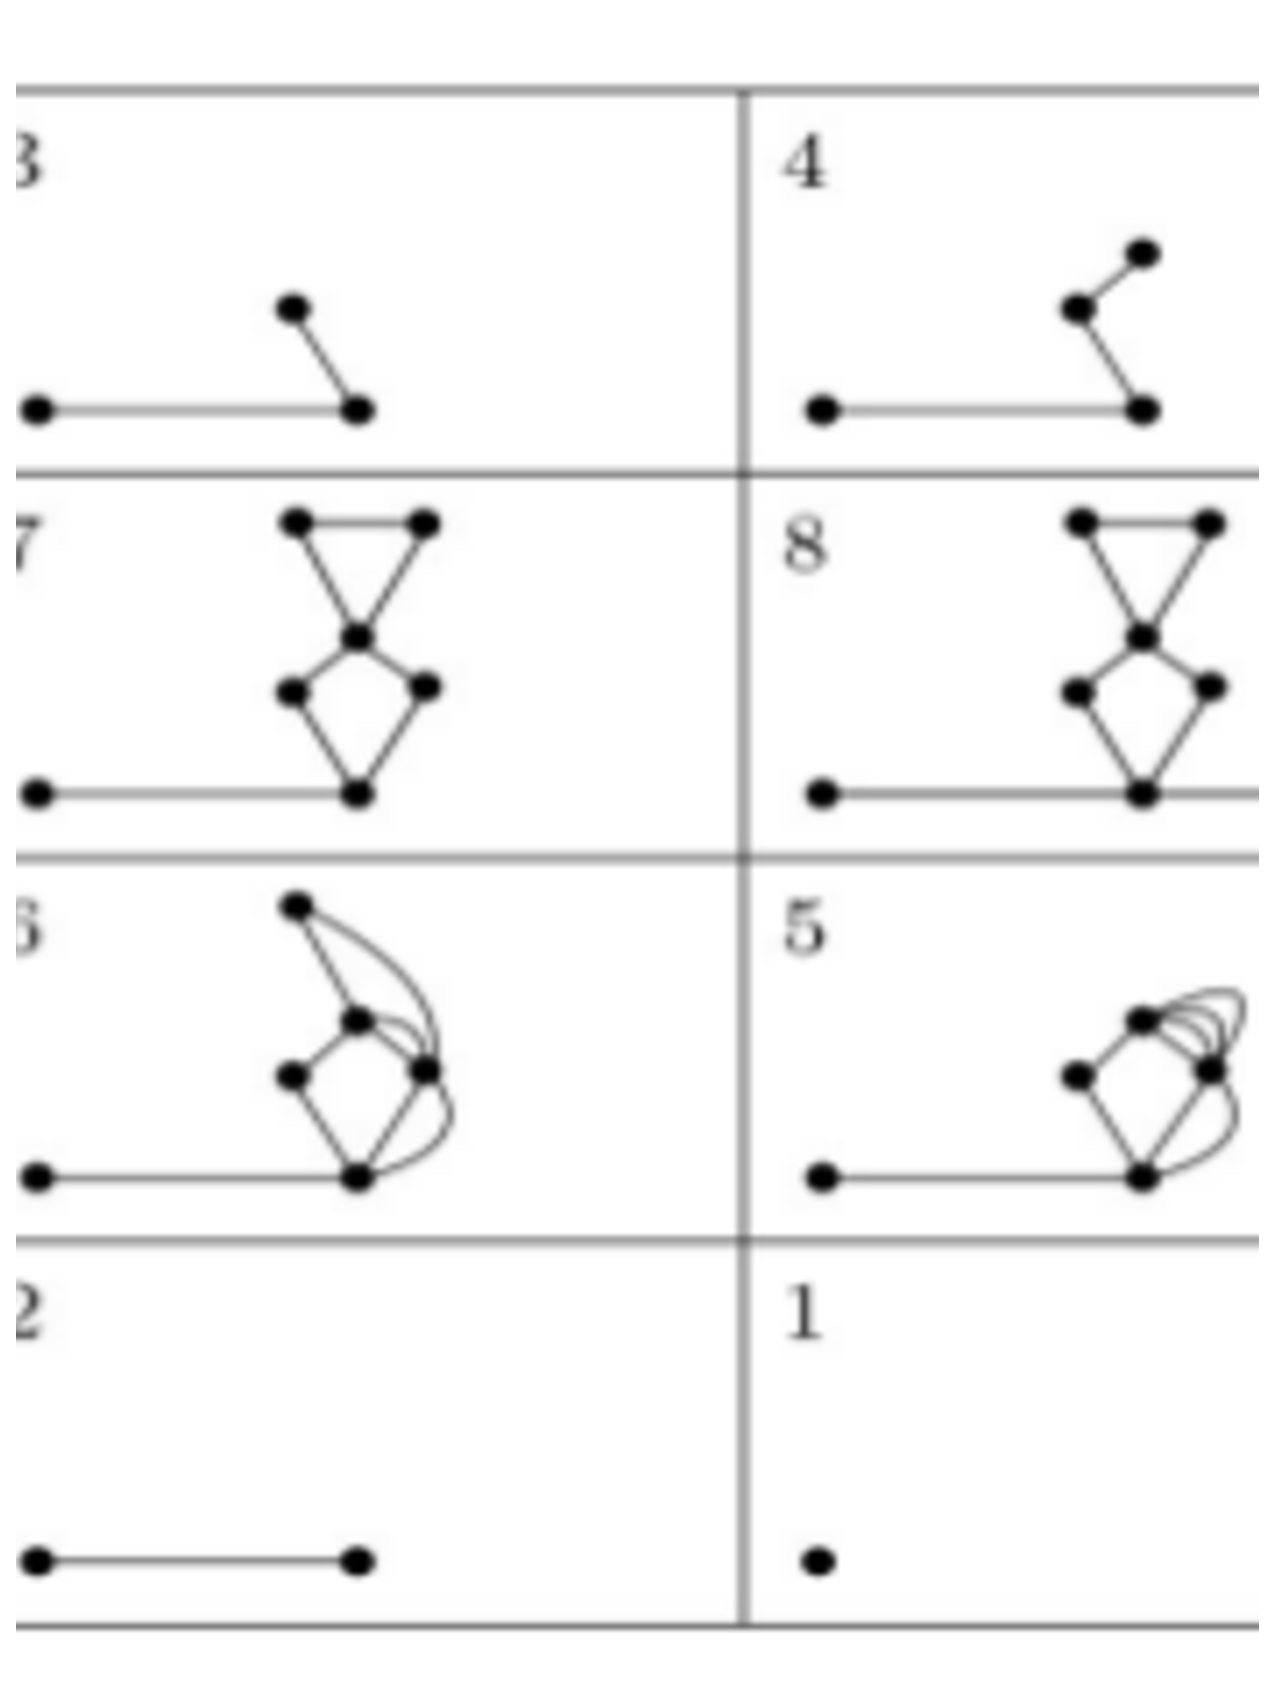
\includegraphics[scale=0.2,center]{./images/extended-ph.eps}

\subsection{Extended Persistence and Branch Decomposition}

In this subsection we will tackle a claim that has been made in the paper that first introduced branch decomposition of contour trees. The claims is the following : "... we define the persistence of a branch to be the greater of its length and the persistence of each of it children. This definition differs from the definition of persistence given in [10] because it takes into consideration the topological obstructions. " \cite{ct-branch-decomp}. In that quote the reference to "[10]" is to the original paper that introduced persistent homology \cite{persistence-original}.

Let us unpack the claim piece by piece. Firstly the paper only redefines how the persistence of the branches is computed and branches are pair of critical points. Therefore for this to be equivalent to the persistence pairs, both methods must  produce equivalent pairs. It is clear from this definition that the actual persistence pairings stay the same, we only compute the persistence value in a different way. What we will aim to show is that the pairings produced by persistent homology are in themselves different from the pairings produces by branch decomposition. After this it will not matter how the actual persistence of branches is computed as they are fundamentally different things. Lastly the paper claims that the branch decomposition definition differs from persistent homology in that "it takes into consideration the topological obstructions.". It is not clear exactly what the authors meant by "topological obstructions". These obstructions are not defined in the paper nor in subsequent publications. This does not stop us from working with the definition because we will demonstrate a second way in which persistence differs from branch decomposition.

The first major difference we can find comes from the fact that persistent homology as it was originally defined does not pair all critical points. As we discussed previously the pairings of essential homology classes are not defined because they never die in the filtration. In the case of contour trees we will be dealing will simply connected contractable domains. Such domains have a single connected component and therefore have exactly one essential homology class in the 0th homology. This is the class that is born at the global minimum, or the first simlicial complex in the filtration. In branch decomposition on the other hand all critical points are paired.

This is already of major difference between the two. Furthermore the paper on branch decomposition clearly cites the original paper for persistent homology and not the subsequence paper on extended persistence where this issue is remedied. In fact it cannot reference that paper. The branch decomposition paper has been published in January of 2004 and the paper that clearly defines Extended Persistence as such has been published in January of 2009 \cite{persistence-extended}. There is however more to this story. The concept of pairing critical points unpaired by persistence goes further back than the 2009 paper and can be traced to the paper \cite{extreme-elevation} which was also published in January of 2004. The paper outlines the initial concept of extended persistence in the specific case of 2-manifolds embedded in $\mathbb{R}^3$. This means that the idea of pairing all critical points was present when the claim was made. All of lets us the take this a step further. We will now test whether branch decomposition is equivalent to extended persistence.

We will demonstrate that they are not with a small counter example. This counter example will show that at least one pair in both is necessarily different. In contour trees where the global minimum and the global maximum are not connected via a monotone path branch decomposition cannot by definition pair them as the endpoints of a branch. Extended persistence on the other hand does pair them as the global maximum is the first class in the descending relative filtration that is homologous to the essential class born at the global minimum. To reduce the stress caused by the reader's feverish anticipation of this counter example we will foreshadow that it is a contour tree with a w-structure. This w-structure is what separates the global minimum from the global maximum.

Let us first begin with an example data set show in fig. Let us call that $X$. The contour tree of this data set is shown in fig and a branch decomposition of this contour tree is shown in fig. The ascending filtration of this data set is shown in fig. The ascending filtration consists of nine simplical complexes $\{X_1, X_2, ..., X_9\}$. According to that filtration we can produce the persistence diagram on fig[]. The extended persistence of the 0th is shown in fig. 

According to our extended persistence computation the pair are $(2, 5)$ and $(1, 9)$. The first pair comes from ordinary persistence. We can see on fig [] that a component is born in time $2$ and dies in time $t$. The second pair is of the global minimum and global maximum. It comes from extended persistence. To verity this observe that $H_0(X_9) = \mathbb{Z}$ because there is one one connected component. The next homology group in the sequence in the group is $H_0(X, X^9) = \overset{\sim}{H}_0(X / X^9) = \overset{\sim}{H}_0(X / \{9\}) = \overset{\sim}{H}_0(X) = 0$. It follows that the induced map $i_* : H_0(X_9) \to H_0(X, X^9)$ is the zero map. Therefore the homology class in $H_0(X, X^9)$ that is born at time 1 at the global minimum must die time 9 and so $(1, 9)$ is a pair in extended persistence.

Here is the summary of you findings.

\begin{itemize}
    \item There is no monotone path between the global minimum and global maximum in the data set.
    \item There is no monotone path between the global minimum and global maximum in the contour tree.
    \item No branch decomposition of the contour tree can pair the global minimum and the global maximum.
    \item Extended persistence pairs the global minimum and the global maximum.
\end{itemize}

This counter examples demonstrates that branch decomposition is not always equivalent to extended persistence. But they are equivalent on some contour trees. Examine the simple contour tree on fig []. Let us now go a step further and demonstrate a whole class of counter examples where they are not equal. This class will be that of all contour trees where there is no monotone path between the global minimum and the global maximum. It is already clear that in the branch decomposition of such trees they will not be paired. All we have to do is prove that extended persistence does pair them.



\begin{figure}[h]%
    \centering
    \subfloat[Original Data Set]{{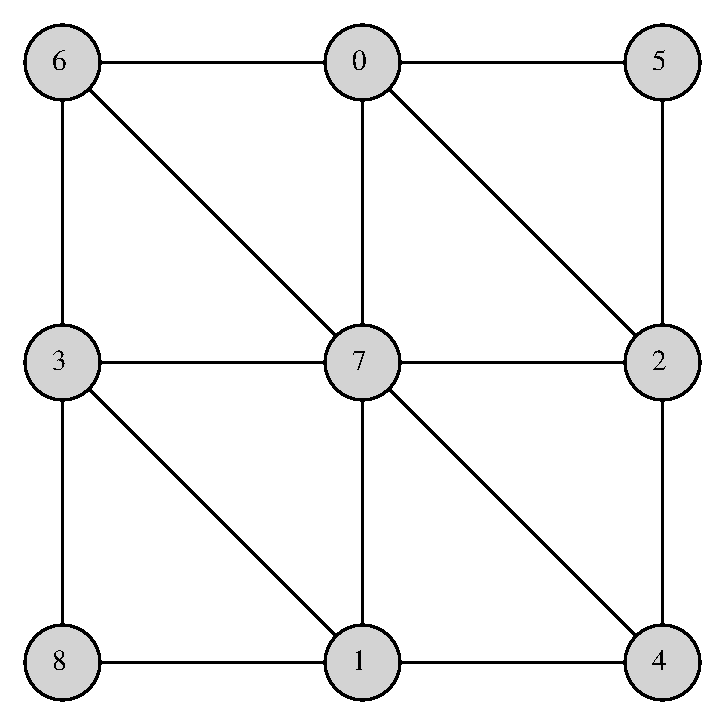
\includegraphics[scale=0.4]{./images/chapter4/w3x3-grid.eps}}}%
    \qquad
    \subfloat[Contour Tree]{{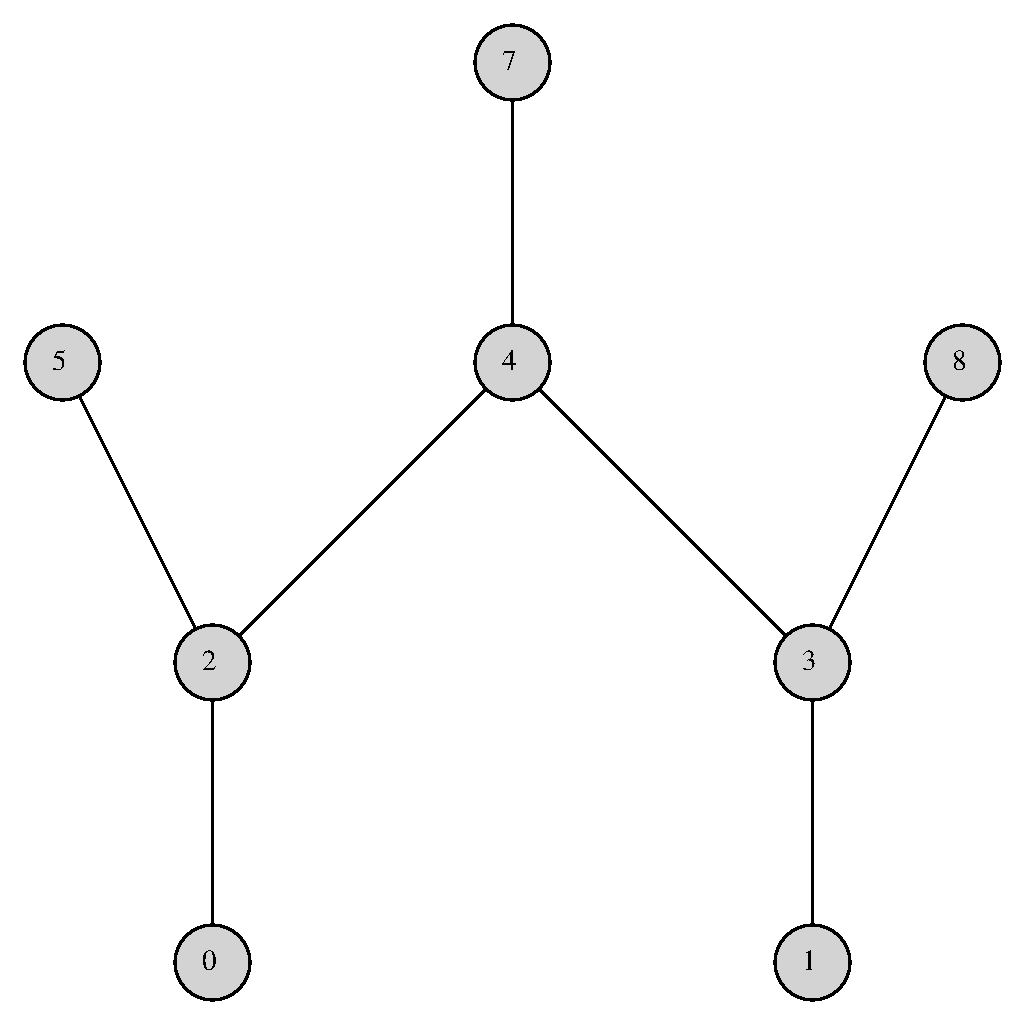
\includegraphics[scale=0.3]{./images/w3x3.eps}}}%
    \qquad
    \subfloat[Branch Decomposition.]{{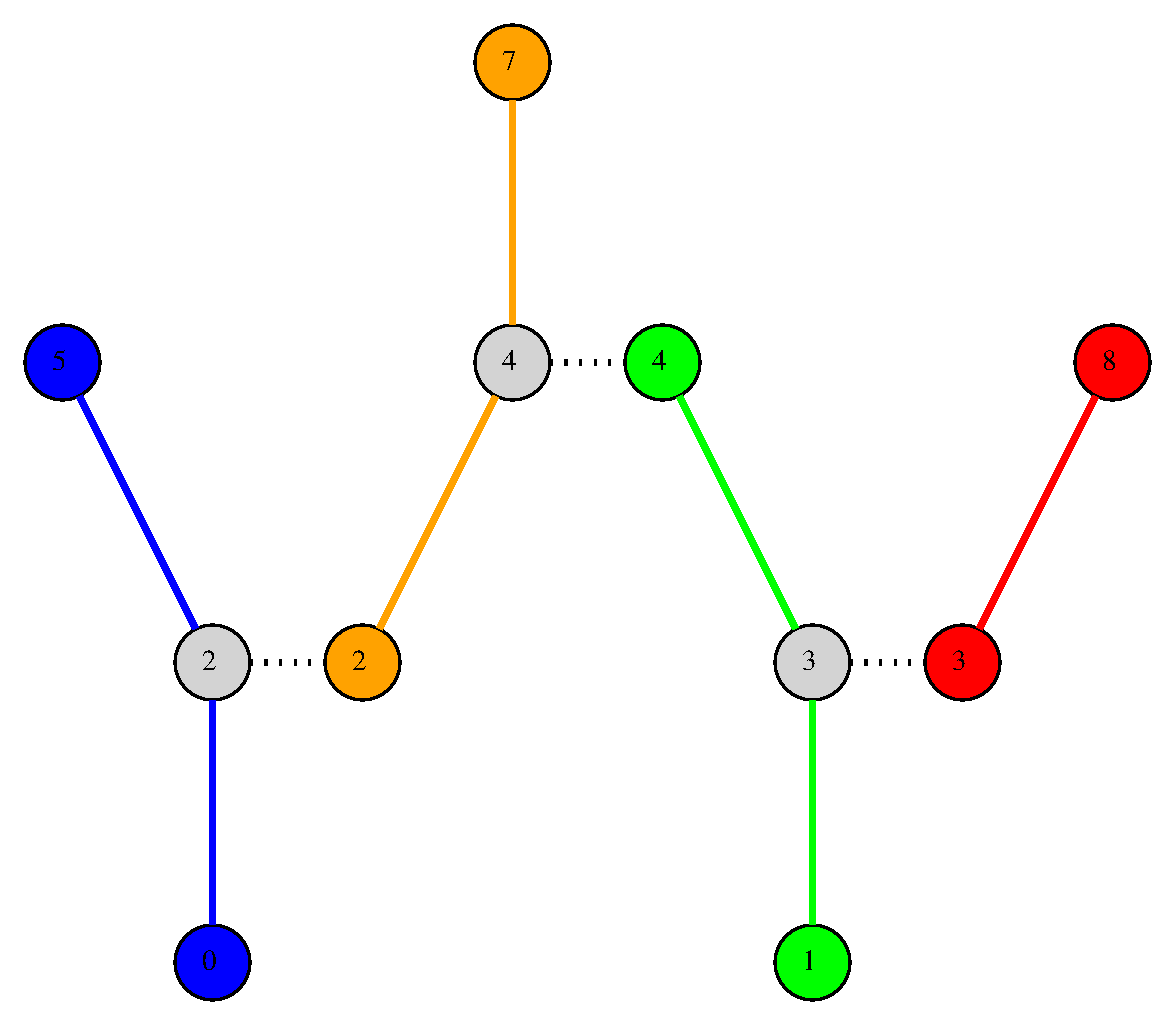
\includegraphics[scale=0.3]{./images/branch-decomposition-W3x3.eps}}}%
    \caption{Branch Decomposition of the Contour tree.}%
    \label{fig:example}%
\end{figure}

Here is the ascending filtration.

\begin{figure}[h]%
    \centering
    \includegraphics[scale=0.08]{./images/chapter4/asc-filt.eps}%
    \caption{Ascending filtration of the Simplical Complex}%
    \label{fig:filt-sc}%
\end{figure}

\begin{figure}[h]%
    \centering
    
\includegraphics[scale=0.08]{./images/chapter4/ph.eps}%
    \caption{Extended Persistence of the Simplical Complex}%
    \label{fig:filt-sc}%
\end{figure}


\subsection{Extended Persistence on Path-Connected Domains}

The final step we take on this journey will be to prove the following original and more general result.

\begin{prop} In the extended persistence of filtration a Morse function with a Path-Connected domain the global minimum pairs with the global maximum in the 0th homology \end{prop}

\begin{proof}
    Let $M$ be a Path-Connected domain and let $M_1 \subseteq M_2 \subseteq ... \subseteq M_n$ be a filtration of $M$. This filtration induces etended persistence 

$$ 0 = H_0(M_{c_1}) \rightarrow ... \rightarrow H_0(M_{c_n}) = H_0(M) = H_0(M, M^{c_n}) \rightarrow ... \rightarrow H_0(M, M^{c_{1}}) = 0.$$

As $M$ is Path-Connected it has one path-connected component and therefore $H_0(M) = H_0(M_0) \simeq  \mathbb{Z}_2$.  Our aim here will be to show that all of the $H_0(M, M^{c_i})$ are trivial. This will mean that the single homology class that exists in $H_0(M)$ will die at $H_0(M, M^{c_n})$ which is exactly the global maximum.


% @TODO Define Excision
% @TODO  Add the thing where this holds - H_n(M / M^{c_i}, pt) = \overset{\sim}{H}_n(M / M^{c_i})
As a corollary of the Excision Theorem we have that

$$H_0(M, M^{c_i}) = H_0(M / M^{c_i}, pt) = \overset{\sim}{H}_0(M / M^{c_i})$$  

where $pt = M^{c_i} / M^{c_i}$.

Now let us explore the reduced homology of the topological space $M / M^{c_i}$. We will show that is it path-connected and therefore the reduced homology is trivial.


% @TODO Add quote
By definition $M$ is path connected. Consider the function $\pi: M \to M/ M^{c_i}$ that takes a point to it's equivalent class. By point set topology [] we know that $\pi$ is continuous. We can also infer that $\pi$ is surjective. Indeed there there is no equivalence class that no point maps to. Furthermore the continuous image of a path connected is connected by []. As we have that $M$ is path-connected therefore $\pi(M) = M / M^{c_i}$ is path-connected. 

By [] we have that $H_0(M / M^{c_i}) = \mathbb{Z}_2$ and by [] that $H_0(M / M^{c_i}) = \overset{\sim}{H}_0(M / M^{c_i}) \bigoplus \mathbb{Z}_2$

We can conclude that $H_0(M, M^{c_i}) = \overset{\sim}{H}_0(M / M^{c_i}) = 0$

Therefore the map induced by the inclusion of the pairs $(M, \emptyset) \to (M, M^{c_n})$ will map the essential homology class of $H_0(M_n)$ to zero. This mean that the global minimum pairs with the global maximum.

\end{proof}

Following this proposition we can only conclude that in any contractable domain with a w-structure that separates the global minimum with the global maximum branch decomposition is not the same as extended persistence.

\subsection{Extended Persistence and Join/Split Trees - Thoughts on future directions}

What we have uncovered is not the complete story. There is a deeper connection between extended persistence and contour trees in general. If we look at alternative algorithms for constructing the 0th homology specifically we can see that the extended persistence of an ascending filtration is equivalent to branch decomposition of the join tree and the extended persistence is equivalent to a branch decomposition of the split tree.

Going back to the claim made \cite{ct-branch-decomp} we see that there is truth to it if we adjust it to extended persistence and apply specifically to join and split trees. Here future questions that arise based on this fact.

\begin{itemize}
    \item By using the persistence pairs on other homology group we can produce split and join tree for the cycles, void, etc... We can them combine them like we combine the join and split trees for the contour. What kind of a structure does that yield?
    \item Can we compute the contour tree directly from homology. Can we find a natural continuous function between the level sets of a filtration. Would the persistence of this sequence be equivalent to the contour tree. In higher dimensions would be equivalent to the previous point?
    \item Who killed Laura Palmer and will the new Twin Peaks be good?
\end{itemize}



%In this final section we will present examples for how extended persistence on the 0th homology is actually equivalent to computing join and split tree.

%*Don't know if I can prove this yet, but it probably won't be too hard. But then again it may be.*

%*Should I keep this or not?*







% @TODO Check spelling in references.



%Let us now restrict $M$ to be compact and contractable. This will ensure that the Reeb Graph of $M$ is a Contour Tree. We would like to tackle the claim made in \cite{ct-branch-decomp} that the persistent homology pairs are equivalent to branch decomposition pairs. We can immediately see that this claim is either false of ill-defined. The major reason for this is that essential homology classes do not get paired. But in the branch decomposition schemes all critical points are paired.

%There is however yet more reason to pursue this. Slightly after the paper of branch decomposition was published, there emerged a way to extend the persistent homology scheme so that all critical points get paired. Using this will allows us to directly compare it to the branch decomposition of a contour tree. 




%Lastly we will not that we cannot take into account the



%Explain the claim that has been made and quote it directly.

%Show why it is flawed in the first place.

%Show why it's not equivalent to it.



%* Most of this sections will be pictures this is why it is not written up properly *

%Now let us examine the relation of extended persistence to branch decomposition. Here is an example branch decomposition of a contour tree of the following 3x3 grid dataset. It is not possible for the branch decomposition to pair the global maximum with the global minimum. There is no monotone path between them. To show that no branch decomposition of a contour tree is equivalent to the extended persistence of the dataset I will demonstrate that extended persistence necessarily pair the global minimum with the global maximum. 

%*Show the extended persistence filtration of the W3x3*
%*Show the branch decomposition*


% @TODO Add quote
%As you can see these methods produce very different pairings. We will conclude that the claims made in [] are either false of not well defined. The correct way to phrase this is the following. "Our definition of persistence is quivalent to extended persistence for the join and split trees. It is not directly applicable in the case of the contour tree itself in terms of the formalism it's built on".


%It so happens that a w-structure that this dissertation is devoted to causes not only computational difficulties, but also serve as counterexamples to pose theoretical difficulties as well. To further cement statement we will us show a more general general result in the following chapter which holds for all filtrations of path-connected spaces.


%The maps in the ascending filtrations are induced via the inclusion maps between the nested spaces $M_i \subseteq M_j$  where $i \le j$. The more interesting case if between the relative homology groups. First of all the isomorphism between $H_n(M) = H_n(M, M^{c_n})$ comes from that fact that $M^{c_n} = \emptyset$ and quotienting by the empty sets leaves a group unchanged. The show where the consecutive maps come from we will give the following example.

%Let $X$ be a simplical complex, $B \subset X$ be a subcomplex of $X$ and $A \subset B$ be a subcomplex of $B$. Then we can find a natural map from $H_n(X, A)$ to $H_n(X, B)$ induced by the inclusion from $A$ to $B$. Let us write out $C_n(X), C_n(A), C_n(B)$ through their generator simplicies.

% @TODO Fix these brackets
%$$ C_n(X) = <a_1, a_2, ..., a_k, ..., a_l, ..., a_n> $$
%$$ C_n(A) = <a_l, ..., a_n>$$
%$$ C_n(B) = <a_k, ..., a_l, ..., a_n>$$


%Then the relative chains are generated by:

%$$ C_n(X, A) = <a_1, ..., a_k, ..., a_{l-1}>$$
%$$ C_n(X, B) = <a_1, ..., a_{k-1}>$$


% @TODO Show it is a chain map

%Where we can introduce a natural inclusion map $f : C_n(X, A) \to C_n(X, B)$ where $f(a_i) = a_i$ when $i < k$ and $f(a_i) = 0$ when $i \ge k$. The map $f$ is well defined as an inclusion map and furthermore it is a chain map. Chain maps induce linear maps on the homology. Therefore we obtain the map $f_* : H_n(X, A) \to H_n(X, B)$ where $f_*([\alpha]) = [f(\alpha)]$. Where the brackets denote the homology quotient classes in $H_n(X, A) \text{ and } H_n(X, B)$ respectively.

%Now let us to back to the descending filtration of $M$. We have 

%Let us go back extended persistence. In the descending filtration of the relative homology we have the scenario we just described. Therefore as there is an inclusion function for between every $M^{c_i}$ and every $M^{c_j}$ where $i \ge j$ and this induces a linear map between every $H_n(M, M^{c_i})$ and $H_n(M, M^{c_j})$.

%We have developed all this mathematical machinery

%-- Give some intuition behind this.

%-- Show how this is used on an example.

%-- Give an algorithm for computing it.

%-- Explain how the algorithm is connected to the computation.

%\section{Persistent Homology and the Contour Tree}

%-- Say some general things about how we are going to relate the two and what we shall accomplish in this chapter.

%\subsection{Join and Split Trees}

%Show that the computation of the ascending filtration and descending filtration is equivalent to the join and split tree of a contractable domain.

%Show the it is equivalent to branch decomposition of the join and split tree.

%Show that extended persistence pairing are not equivalent to branch decomposition pairing. Say the paper is either wrong or had something else in mind which is not clarified well enough.

%Emerge victorious and have the plebeians chant you name in the streets. All Hail Petros all hail Petros.
